\section{Evaluation}
\label{sec:eval}

We have implemented our approach in \toolname: a system for
repairing parse errors for \python at its entirety. Next,
we describe our implementation and an evaluation that addresses three
questions:

\begin{itemize}
    \item \textbf{RQ1}: How \emph{accurate} are \toolname's predicted error production rules?
                        (\S~\ref{sec:eval:accuracy})
    \item \textbf{RQ2}: How \emph{precisely} can \toolname repair parse errors?
                        (\S~\ref{sec:eval:precise})
    \item \textbf{RQ3}: How \emph{efficiently} can \toolname repair parse errors?
                        (\S~\ref{sec:eval:efficiency})
    \item \textbf{RQ4}: How \emph{useful} are \toolname's suggested repairs?
                        (\S~\ref{sec:eval:useful})
    % \item \textbf{RQ4}: How \emph{precise} are \toolname's template fixes?
    %                     (\S~\ref{sec:eval:template_quality})

\end{itemize}

% \subsection{Implementation} \label{sec:eval:gen_method}

\mypara{Training Dataset}
%
For our evaluation, we use a \python dataset gathered from
PythonTutor.com~\citep{Guo2013} between 2017 and 2018, previously used in
related work \citep{Endres2019,Cosman2020}. Each program which throws an
uncaught Python exception is paired with the next program by the same user that
does not crash, under the assumption that the latter is the fixed version of the
former. We discard pairs where the difference between crashing and fixed
versions is too high (more than a standard deviation above average), since these
are usually unrelated submissions or complete refactorings. We also discard
submissions that violate PythonTutor's policies (e.g., those using forbidden
libraries). Ultimately, the dataset used in this evaluation contains almost a
million usable program pairs, representing students from dozens of universities
(PythonTutor has been used in many introductory courses~\citep{Guo2013}) as well
as non-traditional novices.

\mypara{Dataset labeling}
%
\toolname represents each program with its abstracted token sequence $t^a$ for
the training procedure. For the full set of \python there are \emph{360 terminal
error production rules} that \toolname's has to predict from.

% \mypara{Dataset Cleaning}
% %
% We extract fixes as expressions replacements over a program pair using
% $\diffsym$ A disadvantage of using $\diffsym$s with this dataset is that some
% students may have made many, potentially unrelated, changes between
% compilations; at some point the ``fix'' becomes a ``rewrite''. These rewrites
% can lead to meaningless fix templates and error locations. We discard such
% outliers when the fraction of subexpressions that have changed in a program is
% more than one standard deviation above the mean, establishing a
% $\diffsym$ threshold of 40\%. We also discard programs that have changes in 5 or
% more locations, noting that even state-of-the-art multi-location repair
% techniques cannot reproduce such ``fixes'' \citep{Saha_2019}. The discarded
% changes account for roughly 32\% of each dataset, leaving 2,475 program pairs
% for \SPRING and 2,177 pairs for \FALL. Throughout, we use \SPRING as a training
% set and \FALL as a test set.

% \mypara{\dnn based Classifier}
% %
% \toolname's template prediction uses a multi-layer neural network \dnn based
% classifier with three fully-connected hidden layers of 512 neurons. The neurons
% use rectified linear units (ReLU) as their activation function
% \citep{Nair2010-xg}.
% %
% The \dnn was trained using \emph{early stopping} \citep{Hastie2009-bn}: training
% is stopped when the accuracy on a distinct small part of the training set is not
% improved after a certain amount of epochs (5 epochs, in our implementation).
% %
% We set the maximum number of epochs to 200.
% %
% We used the \textsc{Adam} optimizer \citep{Kingma2014-ng},
% a variant of stochastic gradient descent that converges faster.

\subsection{RQ1: Accuracy}
\label{sec:eval:accuracy}

We consider \toolname's transformer classifiers' accuracy up to the \emph{top
50} error production rules predictions against our original and the final
version of our approach

% colors from http://colorbrewer2.org/?type=sequential&scheme=Blues&n=3
\definecolor{blue1}{HTML}{DEEBF7}
\definecolor{blue2}{HTML}{9ECAE1}
\definecolor{blue3}{HTML}{3182BD}
\definecolor{green1}{HTML}{E5F5E0}
\definecolor{green2}{HTML}{A1D99B}
\definecolor{green3}{HTML}{31A354}

\begin{figure}[t]
  % \begin{minipage}[c]{0.49\linewidth}
    \centering
    \resizebox{0.6\linewidth}{!}{
      \Large
      \begin{tikzpicture}
      \begin{axis}[
        ybar stacked,
        width=1.1\linewidth,
        height=11cm,
        % title={Accuracy of Repair Template Prediction},
        ylabel={Prediction Accuracy (\%)},
        bar width=1cm,
        ymin=0.0,
        ymax=101.0,
        ytick={0.0, 10.0, 20.0, 30.0, 40.0, 50.0, 60.0, 70.0, 80.0, 90.0, 100.0},
        yticklabel={\pgfmathparse{\tick}\pgfmathprintnumber{\pgfmathresult}},
        ytick style={draw=none},
        ymajorgrids = true,
        symbolic x coords={original, abstracted, abstracted-best},
        enlarge x limits=0.3,
        xtick=data,
        xtick style={draw=none},
        xticklabels={\textsc{Original}\xspace, \textsc{Abstracted}\xspace, \textsc{Threshold}\xspace},
        %x tick label style={rotate=45, anchor=north east},
        % x tick label style={font=\small},
        % y tick label style={font=\small},
        reverse legend,
        % transpose legend,
        legend style={legend pos = north east, legend columns=4, font=\small},
      ]

      \addplot[draw=black, fill=blue2, bar shift=-.501cm, postaction= { pattern=dots }] coordinates {(original, 0.0) (abstracted, 0.0) (abstracted-best, 79.28025102961365)};

      \resetstackedplots

      \addplot[draw=black, fill=green2, bar shift=.501cm, postaction= { pattern=dots }] coordinates {(original, 0.0) (abstracted, 0.0) (abstracted-best, 69.82968369829683)};

      \resetstackedplots

      \addplot[draw=black, fill=green1, bar shift=.501cm] coordinates {(original, 12.875536480686696) (abstracted, 58.394160583941606) (abstracted-best, 0.0)};
      \addlegendentry{Top-10}
      \addplot[draw=black, fill=green2, bar shift=.501cm] coordinates {(original, 20.100143061516448) (abstracted, 14.922952149229523) (abstracted-best, 0.0)};
      \addlegendentry{Top-20}
      \addplot[draw=black, fill=green3, bar shift=.501cm] coordinates {(original, 31.974248927038623) (abstracted, 15.49067315490673) (abstracted-best, 0.0)};
      \addlegendentry{Top-50}
      \addlegendimage{empty legend}
      \addlegendentry{Rare:}

      \resetstackedplots

      \addplot[draw=black, fill=blue1, bar shift=-.501cm] coordinates {(original, 56.712132089016514) (abstracted, 72.11217885859972) (abstracted-best, 0.0)};
      \addlegendentry{Top-10}
      \addplot[draw=black, fill=blue2, bar shift=-.501cm] coordinates {(original, 11.769733018835673) (abstracted, 9.335163757599531) (abstracted-best, 0.0)};
      \addlegendentry{Top-20}
      \addplot[draw=black, fill=blue3, bar shift=-.501cm] coordinates {(original, 18.65107852186101) (abstracted, 11.253840622344256) (abstracted-best, 0.0)};
      \addlegendentry{Top-50}
      \addlegendimage{empty legend}
      \addlegendentry{All:}

      \end{axis}
      \end{tikzpicture}
    }
    \caption{
      Results of our error production rule prediction classifiers for the simple original token sequences and their abstracted versions using the PCFG.
    }
    \label{fig:accuracy-results}
  % \end{minipage}
  % \begin{minipage}[c]{0.49\linewidth}
  %   \centering
  %   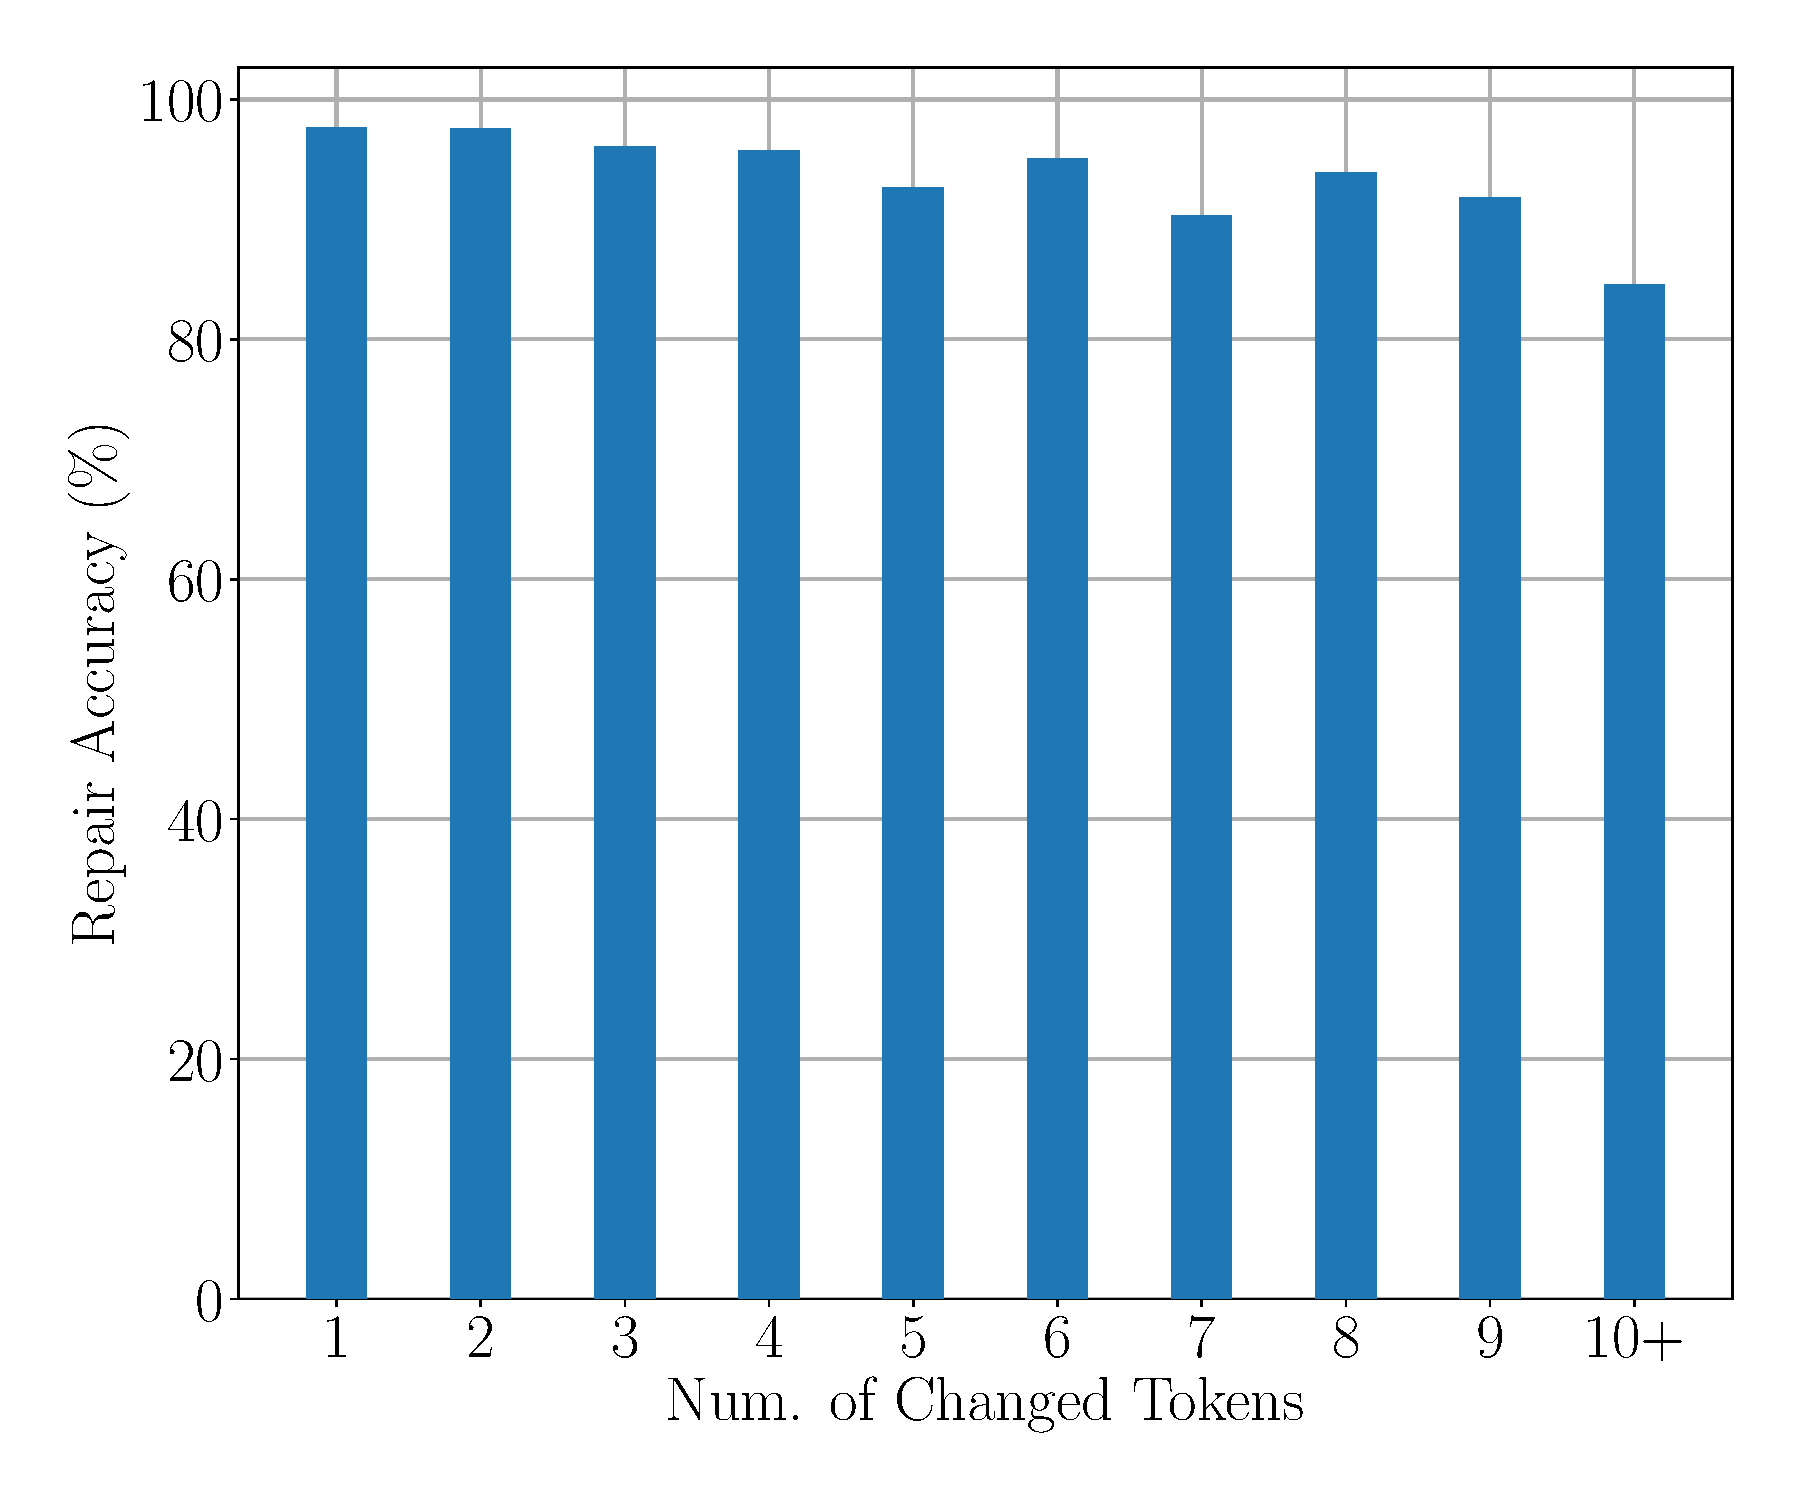
\includegraphics[width=\linewidth]{accuracy-per-change.pdf}
  %   \caption{The repair accuracy for the number of edits needed by the user to repair.}
  %   \label{fig:accuracies-per-changes}
  % \end{minipage}
\end{figure}


\mypara{Results: Accuracy of Error Rule Prediction}
%
\autoref{fig:accuracy-results} shows the accuracy results of our error
production rule prediction experiments. The y-axis describes the fraction of
programs for which the \emph{whole} set of the needed error rules needed to
repair the \emph{erroneous} program was a complete subset of the top-K predicted
rules.
%
The \textsc{Original} version of our transformer classifier didn't consider the
partial parses produced with the PCFG's aid and used the full \textsc{Original}
token sequences, whose results are presented in the first two bars of
\autoref{fig:accuracy-results}. The next two bars show our final results using
the \textsc{Abstracted} token sequences to train the classifier. Finally, the
last two dotted bars show the results for when a \textsc{Threshold} is set in
order to select the predicted error rules, instead of picking the static top-K
ones. The predicted error rule set can have a size anywhere between 1 and a
maximum of 25 (pre-defined by us based on the top-K results).

The blue bars show the accuracy on the full test set of \textsc{All} 15,000
programs, while the green bars show the results on the subset of \textsc{Rare}
programs, \ie the programs that didn't include any of the 50 most popular error
rules, that amount only for 4.8\% of our test set.

The \textsc{Original} predictor, even with the Top-50 predicted error rules is
less accurate than the Top-20 predictions of the \textsc{Abstracted}, with an
accuracy of 73.96\%, which drops to 51.16\% and 32.34\% respectively for the
Top-20 and Top-10 predictions. The \textsc{Abstracted} predictor significantly
outperforms the \textsc{Original} predictor with a 72.08\% Top-10 accuracy,
81.08\% Top-20 accuracy and 92.13\% Top-10 accuracy.

The \textsc{Threshold} predictions are almost as accurate as the
\textsc{Abstracted} Top-20 predictions with an accuracy of 79.46\% and a median
number of selected error rules of 12 (average 13.9). This could potentially mean
that this predictor is a valid alternative for the static Top-20 predictions.

Finally, we observe that our \textsc{Abstracted} classifiers generalize
efficiently for our dataset of erroneous Python programs and is almost as
accurate as the rest of the dataset with a 74.11\% Top-20 accuracy (85.69\%
Top-50 accuracy). The same holds for the \textsc{Threshold} predictions with a
72.46\% accuracy.

\begin{framed}
  \noindent \toolname's transformer classifier learns to encode programs with
  syntax errors and select candidate error production rules for them
  effectively, yielding \emph{high accuracies}. By abstracting the tokens
  sequences, \toolname is able to \emph{generalize} better and make more
  accurate predictions with a \emph{81.08\% Top-20 accuracy}.
\end{framed}


\subsection{RQ2: Repaired Program Preciseness}
\label{sec:eval:precise}

\begin{table}[t]
  \centering
  \begin{tabular}{l||cccc}
    Rules Approach                 & Parse Accuracy & User Parse Rate & Parse time & Speedup \\
    \hline
    20 Most Popular                & 76.84\% & N/A     & 8.2 sec  & 38.6 sec \\
    50 Most Popular                & 83.24\% & N/A     & 13.8 sec & 29.2 sec \\
    Top-20 (\textsc{All-Parses})   & 79.18\% & 36.40\% & 3.3 sec  & 46.3 sec \\
    Top-20 (\textsc{Minimum-Cost}) & 91.57\% & 19.03\% & 42.4 sec & 12.9 sec \\
  \end{tabular}
  \caption{Experimental results of \toolname's repair approaches.}
  \label{tab:seq2parse_full_results}
\end{table}

Next we evaluate \toolname's end-to-end accuracy and preciseness in generating
valid parses for programs with syntax errors. For all of our tests we limit the
\toolname's parsing to \emph{5 mins} and run our experiments on \emph{15,000
erroneous programs} from our dataset. The rest of the dataset was used to train
our transformer classifiers, and specifically here the \textsc{Abstracted}
classifier.

We compare our \emph{two versions} of our implementation of \toolname
(\textsc{All-Parses} and \textsc{Minimum-Cost}) against two versions of the
error-correcting parser with a static selection of the 20 and 50 most popular
error production rules in our training set. We make this comparison because we
observe in our training set that the 50 most of popular error rules are used for
parsing as much as \emph{86\%} of the dataset.

Our \textsc{All-Parses} ECEP and \textsc{Minimum-Cost} ECEP both use the
\emph{Top-20 predictions} from our \textsc{Abstracted} classifier to generate
parses and thus generate full program repairs. The \textsc{All-Parses} ECEP
keeps internally all possible states that arise from using the predicted error
rules and having a maximum repair cost of 2 edits (\ie a maximum of 2
insertions, deletions or replacements). The \textsc{Minimum-Cost} version
however keeps always the minimum-edit repair and discards all other states that
may lead to a higher cost. This allows for a higher maximum cost of 10 edits.
Finally, while \textsc{All-Parses} can generate a large number of repairs, we
keep only the top 3 repairs after filtering with a static code checker
(\textsc{Pylint} \citep{pylint2022}) as most developers will consider at most five
suggestions before falling back to manual debugging \citep{Kochhar2016-oc,
Parnin2011-ce}.

\autoref{tab:seq2parse_full_results} shows the percentage of test programs that
each of these four versions can parse successfully (\ie the parse accuracy) and
the amount of parses that match the one that user compiled. We observe that both
of the Top-20 predictions versions outperform the 20 most popular ECEP
(76.84\%), while 50 most popular falls in between them with 83.24\% parse
accuracy. The \textsc{All-Parses} ECEP achieves slightly less pase accuracy with
79.18\%, however it manages to generate the user fix 36.40\% of the times, \ie
more than one out of three programs with syntax errors. That number decreases to
19.03\% when we consider the \textsc{Minimum-Cost} ECEP, which still an amazing
result, if we also consider the higher total parse accuracy of 91.57\%.

\begin{framed}
  \noindent \toolname can \emph{generate parses} for \emph{80\%} of our tests
  within 4 secs for the majority of them, while also generating \emph{the user
  fix in more than 1 out 3 of the cases}.
\end{framed}

% \subsection{RQ2: Efficiency}
% \label{sec:eval:efficiency}
% \label{subsec:eval:man_rep_qual_eval}

% Next we evaluate \toolname's efficiency by measuring how many programs it is
% able to generate a (well-typed) repair for.
% %
% We limit the synthesizer to 90 seconds. (In general the procedure is
% undecidable, and we conjecture that a longer timeout will diminish the practical
% usability for novices.)
% %
% Recall that the repair synthesis algorithm is guided by the repair template
% predictions.
% %
% We evaluate the efficiency of \toolname by comparing it against a baseline
% \naive implementation that, given the predicted fix location, attempts to
% synthesize a repair from the trivial ``hole'' template.

% \autoref{fig:rite_naive} shows the cumulative distribution function of
% \toolname's and \naive's repair rates over their synthesis time. We observe that
% using the predicted templates for synthesis allows \toolname to generate
% type-correct repairs for almost 70\% of the programs in under 20 seconds, which
% is nearly 12 points higher than the \naive baseline. We also observe that
% \toolname successfully repairs around 10\% more programs than \naive for times
% greater than 20 seconds. While the \naive approach is still able to synthesize
% well-typed repairs relatively quickly, we will see that these repairs are of
% much lower quality than those generated from the predicted templates
% (\S~\ref{sec:eval:template_quality}).

% \begin{framed}
%   \noindent \toolname can generate type-correct repairs for the vast majority of
%   ill-typed programs in under 20 seconds.
% \end{framed}

% \begin{figure}
%   \centering
%   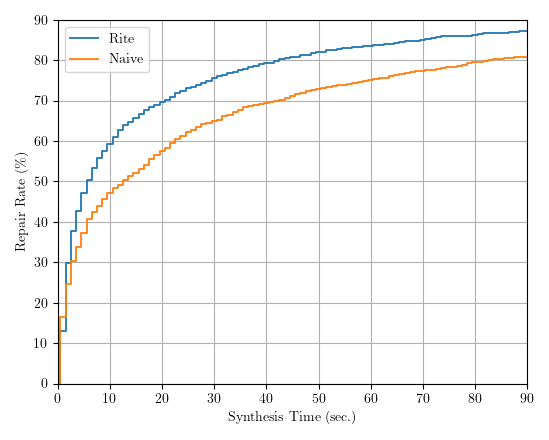
\includegraphics[height=2.3in]{cdf.pdf}
%   \caption{The proportion of the test set that can be repaired within a given time.}
%   \label{fig:rite_naive}
% \end{figure}

% \subsection{RQ3: Usefulness}
% \label{sec:eval:useful}

% The primary outcome is whether the repair-based
% error messages generated by \toolname were actually useful to novices.
% %
% To assess the quality of \toolname's repairs, we conducted an online human
% study with 29 participants.
% %
% Each participant was asked to evaluate the quality of the program fixes
% and their locations against a state-of-the-art baseline
% (\seminal ~\citep{Lerner2007-dt}).
% %
% For each program, beyond the two repairs, participants were presented
% with the original ill-typed program, along with the standard \ocaml
% compiler's error message and a short description of what the original
% author of the program intended it to do.
% %
% From this study, we found that both the edit locations and final
% repairs produced by \toolname were better than
% \seminal's in a statistically significant manner.

% \mypara{User Study Setup}
% %
% Study participants were recruited from two public research
% institutes (names elided for blind review), and was advertised on Twitter.
% %
% Participants had to assess the quality of, and give comprehensible
% bug descriptions for, at least 5 / 10 stimuli. The study took around
% 25 minutes to complete. Participants were compensated by entering a
% drawing for an Amazon Echo voice assistant. There were 29 valid participants.
% %
% We created the stimuli by randomly selecting a corpus of 21 buggy programs
% from the 1834 programs in our dataset where repairs were synthesized.
% %
% From this corpus, each participant was shown 10 randomly-selected buggy
% programs, and two candidate repairs: one generated by \toolname and one
% by \seminal.
% %
% For both algorithms, we used the highest-ranked solution returned.
% %
% Participant were always unaware which tool generated which candidate
% patch.
% %
% Participants were then asked to assess the quality of each
% candidate repair on a Likert scale of 1 to 5 and were asked
% for a binary assessment of the quality of each repair's edit
% location.
% %
% We also collected self-reported estimates of both programming and
% \ocaml-specific experience as well as qualitative data assessing factors
% influencing each participant's subjective judgment of repair quality.
% %
% From the 29 participants, we collected 554 patch quality assessments,
% 277 each for \toolname and \seminal generated repairs.

% %\begin{figure}
% %  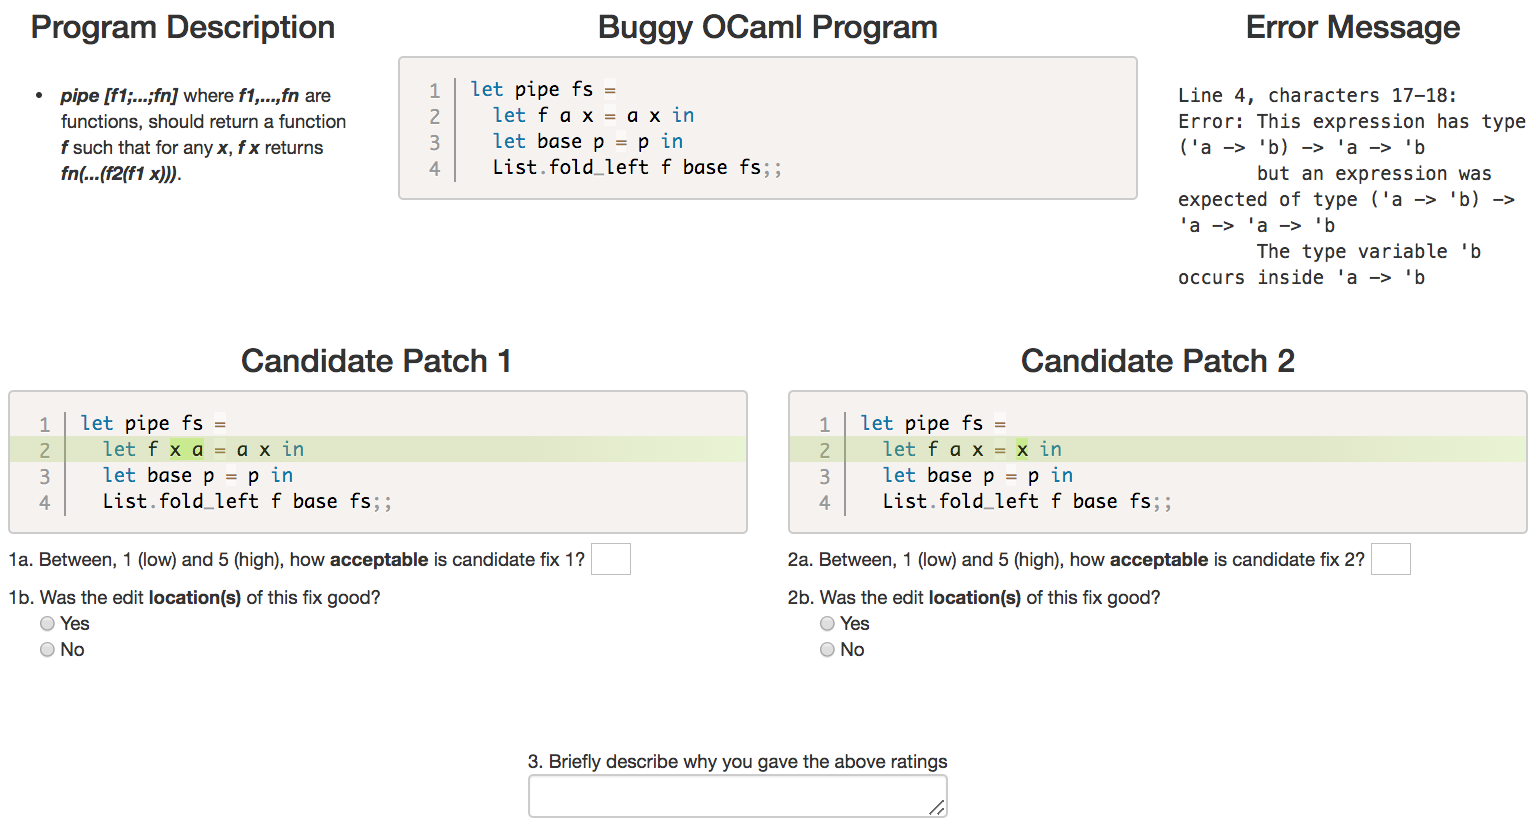
\includegraphics[width=8cm]{SampleStimuli.png}
% %  \caption{A sample stimulus used for assessing repair quality.}
% %  \label{fig:stimulus}
% %\end{figure}

% \mypara{Results}
% %
% In a statistically-significant manner, humans perceive that
% \toolname's fault localization and final repairs are both
% of higher quality than those produced by \seminal ($p=0.030$
% and $p=0.024$ respectively).\footnote{All tests for statistical
% significance used the Wilcoxon signed-rank test.}
% %
% Regarding fault localization, we find that humans agreed
% with \toolname-identified edit locations 81.6\% of the time
% but only agreed with those of \seminal 74.0\% of the time.
% %
% % This 10\% increase is important because \ME{You should explain why this matters.}
% %
% As for the final repair, humans also preferred \toolname's patches
% to those produced by \seminal. Specifically, \toolname's repairs
% achieved an average quality rating of 2.41/5 while \seminal's
% repairs had an average rating of only 2.11/5, a 14\% increase ($p=0.030$),
% showing a statistically-significant improvement over \seminal.

% \begin{figure*}
% \begin{subfigure}[t]{.33\textwidth}
% \centering
% 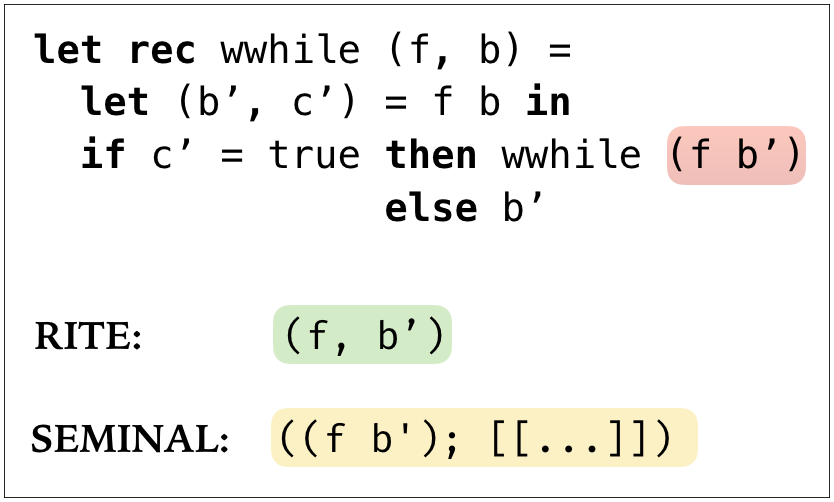
\includegraphics[height=1.4in]{comp1.png}
% \caption{\toolname (4.5/5) better than \seminal(1.1/5) with 12 responses $p=0.002$.}
% \label{subfig:good1}
% \end{subfigure}
% \begin{subfigure}[t]{.33\textwidth}
% \centering
% 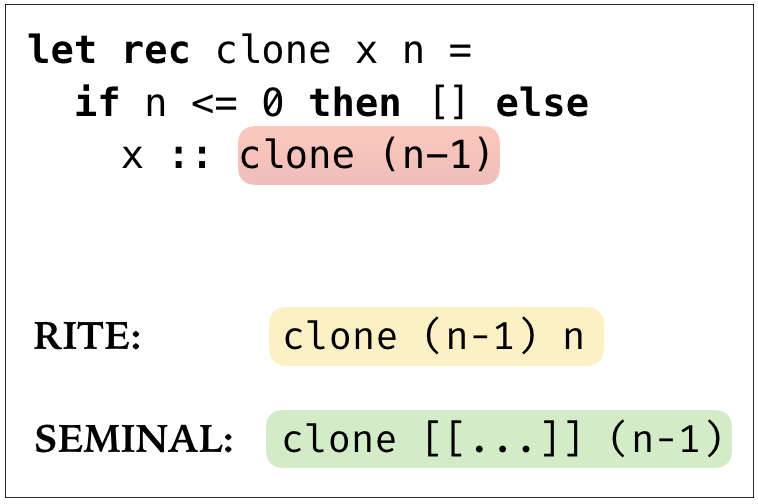
\includegraphics[height=1.4in]{comp2.png}
% \caption{\toolname (1.5/5) worse than \seminal(4.1/5) with 18 responses $p=0.0002$.}
% \label{subfig:bad}
% \end{subfigure}
% \begin{subfigure}[t]{.29\textwidth}
% \centering
% 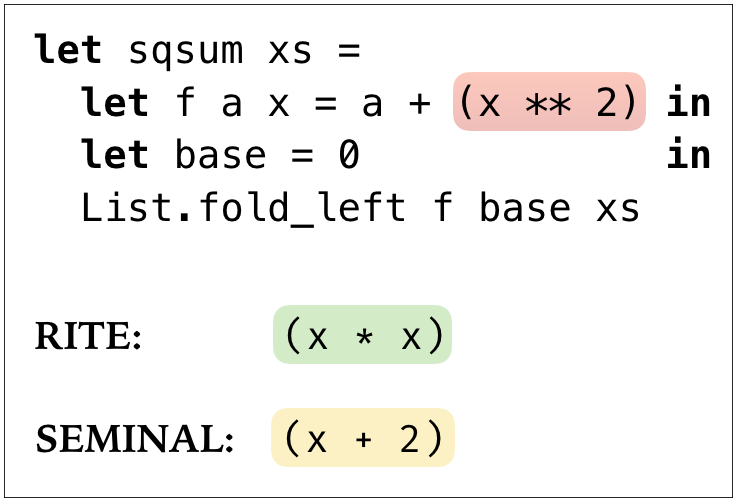
\includegraphics[height=1.4in]{comp3.png}
% \caption{\toolname (4.8/5) better than \seminal(1.2/5) with 17 responses $p=0.0003$.}
% \label{subfig:good2}
% \end{subfigure}
% \end{figure*}

% \mypara{Qualitative Comparison}
% %
% We consider several case studies where there were
% statistically-significant differences between
% the human ratings for \toolname's and \seminal's
% repairs.
% %
% The task in Figure~\ref{subfig:good1} is that
% \texttt{wwhile(f, b)} should return $x$ where
% there exist values $v_0,...,v_n$ such that:
% $b = v_0$, $x = v_n$, and for each $i$ between
% 0 and $n-2$, we have $f v_i = (v_i+1, true)$
% and $f v_n-1 = (v_n, false)$.
% %
% The task in Figure~\ref{subfig:bad} is to
% return a list of \texttt{n} copies of \texttt{x}.
% %
% The task in Figure~\ref{subfig:good2} is to
% return the sum of the squares of the numbers
% in the list \texttt{xs}.
% %
% Humans rated \toolname's repairs better
% for the programs in Fig~\ref{subfig:good1}
% and~\ref{subfig:good2}.
% %
% In both cases, \toolname's found a solution
% which type-checks and conforms to the problem's
% semantic specification.
% %
% \seminal, however, found a repair that was
% either incomplete (\ref{subfig:good1}) or
% semantically incorrect (\ref{subfig:good2}).
% On the other hand, in ~\ref{subfig:bad}, \toolname
% does worse as the \emph{second} parameter should
% be \verb|n-1|. In fact, \toolname's second ranked
% repair is the correct one, but it is equal
% to the first in terms of edit distance.

% \begin{framed}
% \noindent Humans perceive both \toolname's edit locations
%  and final repair quality to be better than those produced
%  by \seminal, a state-of-the-art \ocaml repair tool, in a
%  statistically-significant manner.
% \end{framed}

% \subsection{RQ4: Impact of Templates on Quality}
% \label{sec:eval:template_quality}

% Finally, we seek to evaluate whether \toolname's template-guided
% approach is really at the heart of its effectiveness. To do so,
% as in \S~\ref{sec:eval:efficiency}, we
% compared the results of using \toolname's error messages
% synthesized from predicted templates to those generated by
% a \naive synthesizer that returns the first well-typed term
% (\ie synthesized from the trivial ``hole'' template).

% \mypara{User Study Setup}
% %
% For this user study, we used a corpus of 20 buggy programs randomly chosen in
% \S~\ref{sec:eval:useful}. For each of the programs we generated three messages:
% using \toolname, using \seminal, and using the \naive approach but at the
% \emph{same location} predicted by \toolname. We then randomized and masked the
% order in which the tools' messages were reported, and asked three experts
% (authors of this paper who had not seen the output of any tool for any of those
% instances) to rate the messages as one of ``Good'', ``Ok'' or ``Bad''.

% \mypara{Results}
% %
% Figure~\ref{fig:comparison} summarizes the results of the rating.
% %
% Since each of 20 programs received 3 ratings, there are a
% total of 60 ratings per tool.
% %
% \toolname dominates with 22 Good, 20 Ok and 18 Bad ratings;
% \seminal follows with only 12 Good, 11 Ok and 37 Bad; while
% \naive received no Good scores, 12 Ok scores and a
% dismal 48 Bad scores.
% %
% On average (with Bad = 0, Ok = 0.5, Good = 1),
% \toolname scored 0.53, \seminal 0.30, and \naive
% just 0.1.
% %
% Our rating agreement kappa is 0.54, which is considered ``moderate agreement''.

% \begin{framed}
%   \noindent Repairs generated from predicted
%   templates were of significantly higher quality
%   than those from expert-biased enumeration (\seminal)
%   or \naive enumeration.
% \end{framed}

% \begin{figure}[t]
%   \centering
%   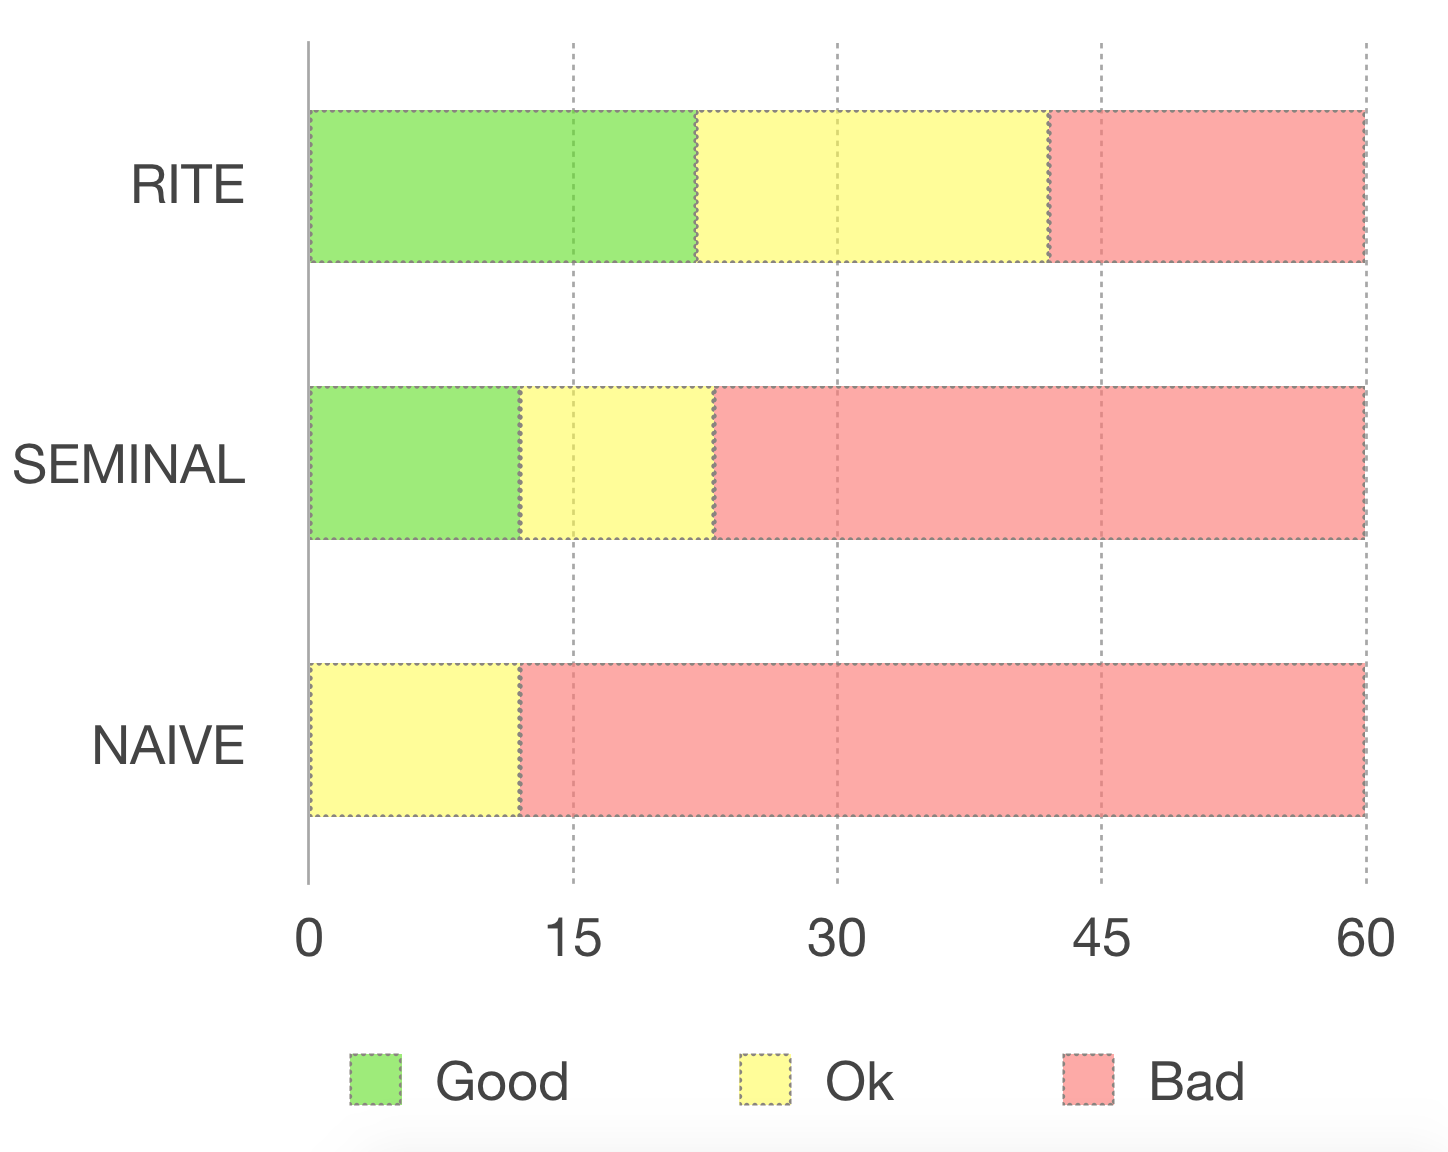
\includegraphics[height=1.5in]{comparison.png}
%   \caption{Rating the errors generated by \toolname, \seminal and \naive enumeration.}
%   \label{fig:comparison}
% \end{figure}
